This chapter presents the findings obtained from the automated benchmark runs conducted across Stage 1 through Stage 5. The results are derived from a \textit{controlled benchmarking prototype} that uses synthetic workloads, local infrastructure, and parameterized proving delays. Accordingly, the reported values should be interpreted as configuration-level measurements that enable relative comparison of design trade-offs, rather than as claims about production mainnet performance.

Before discussing the individual result groups, Figure~\ref{fig:result_analysis_pipeline} summarizes how the benchmark outputs are processed and organized in this chapter. The workflow begins with the automated benchmark runs, continues through metric aggregation and post-processing, and then branches into five stage-specific analyses. These stage-level findings are finally combined into a cross-stage comparison to identify the main performance and cost trade-offs of the RollupX prototype.

\begin{figure}[!htbp]
    \centering
    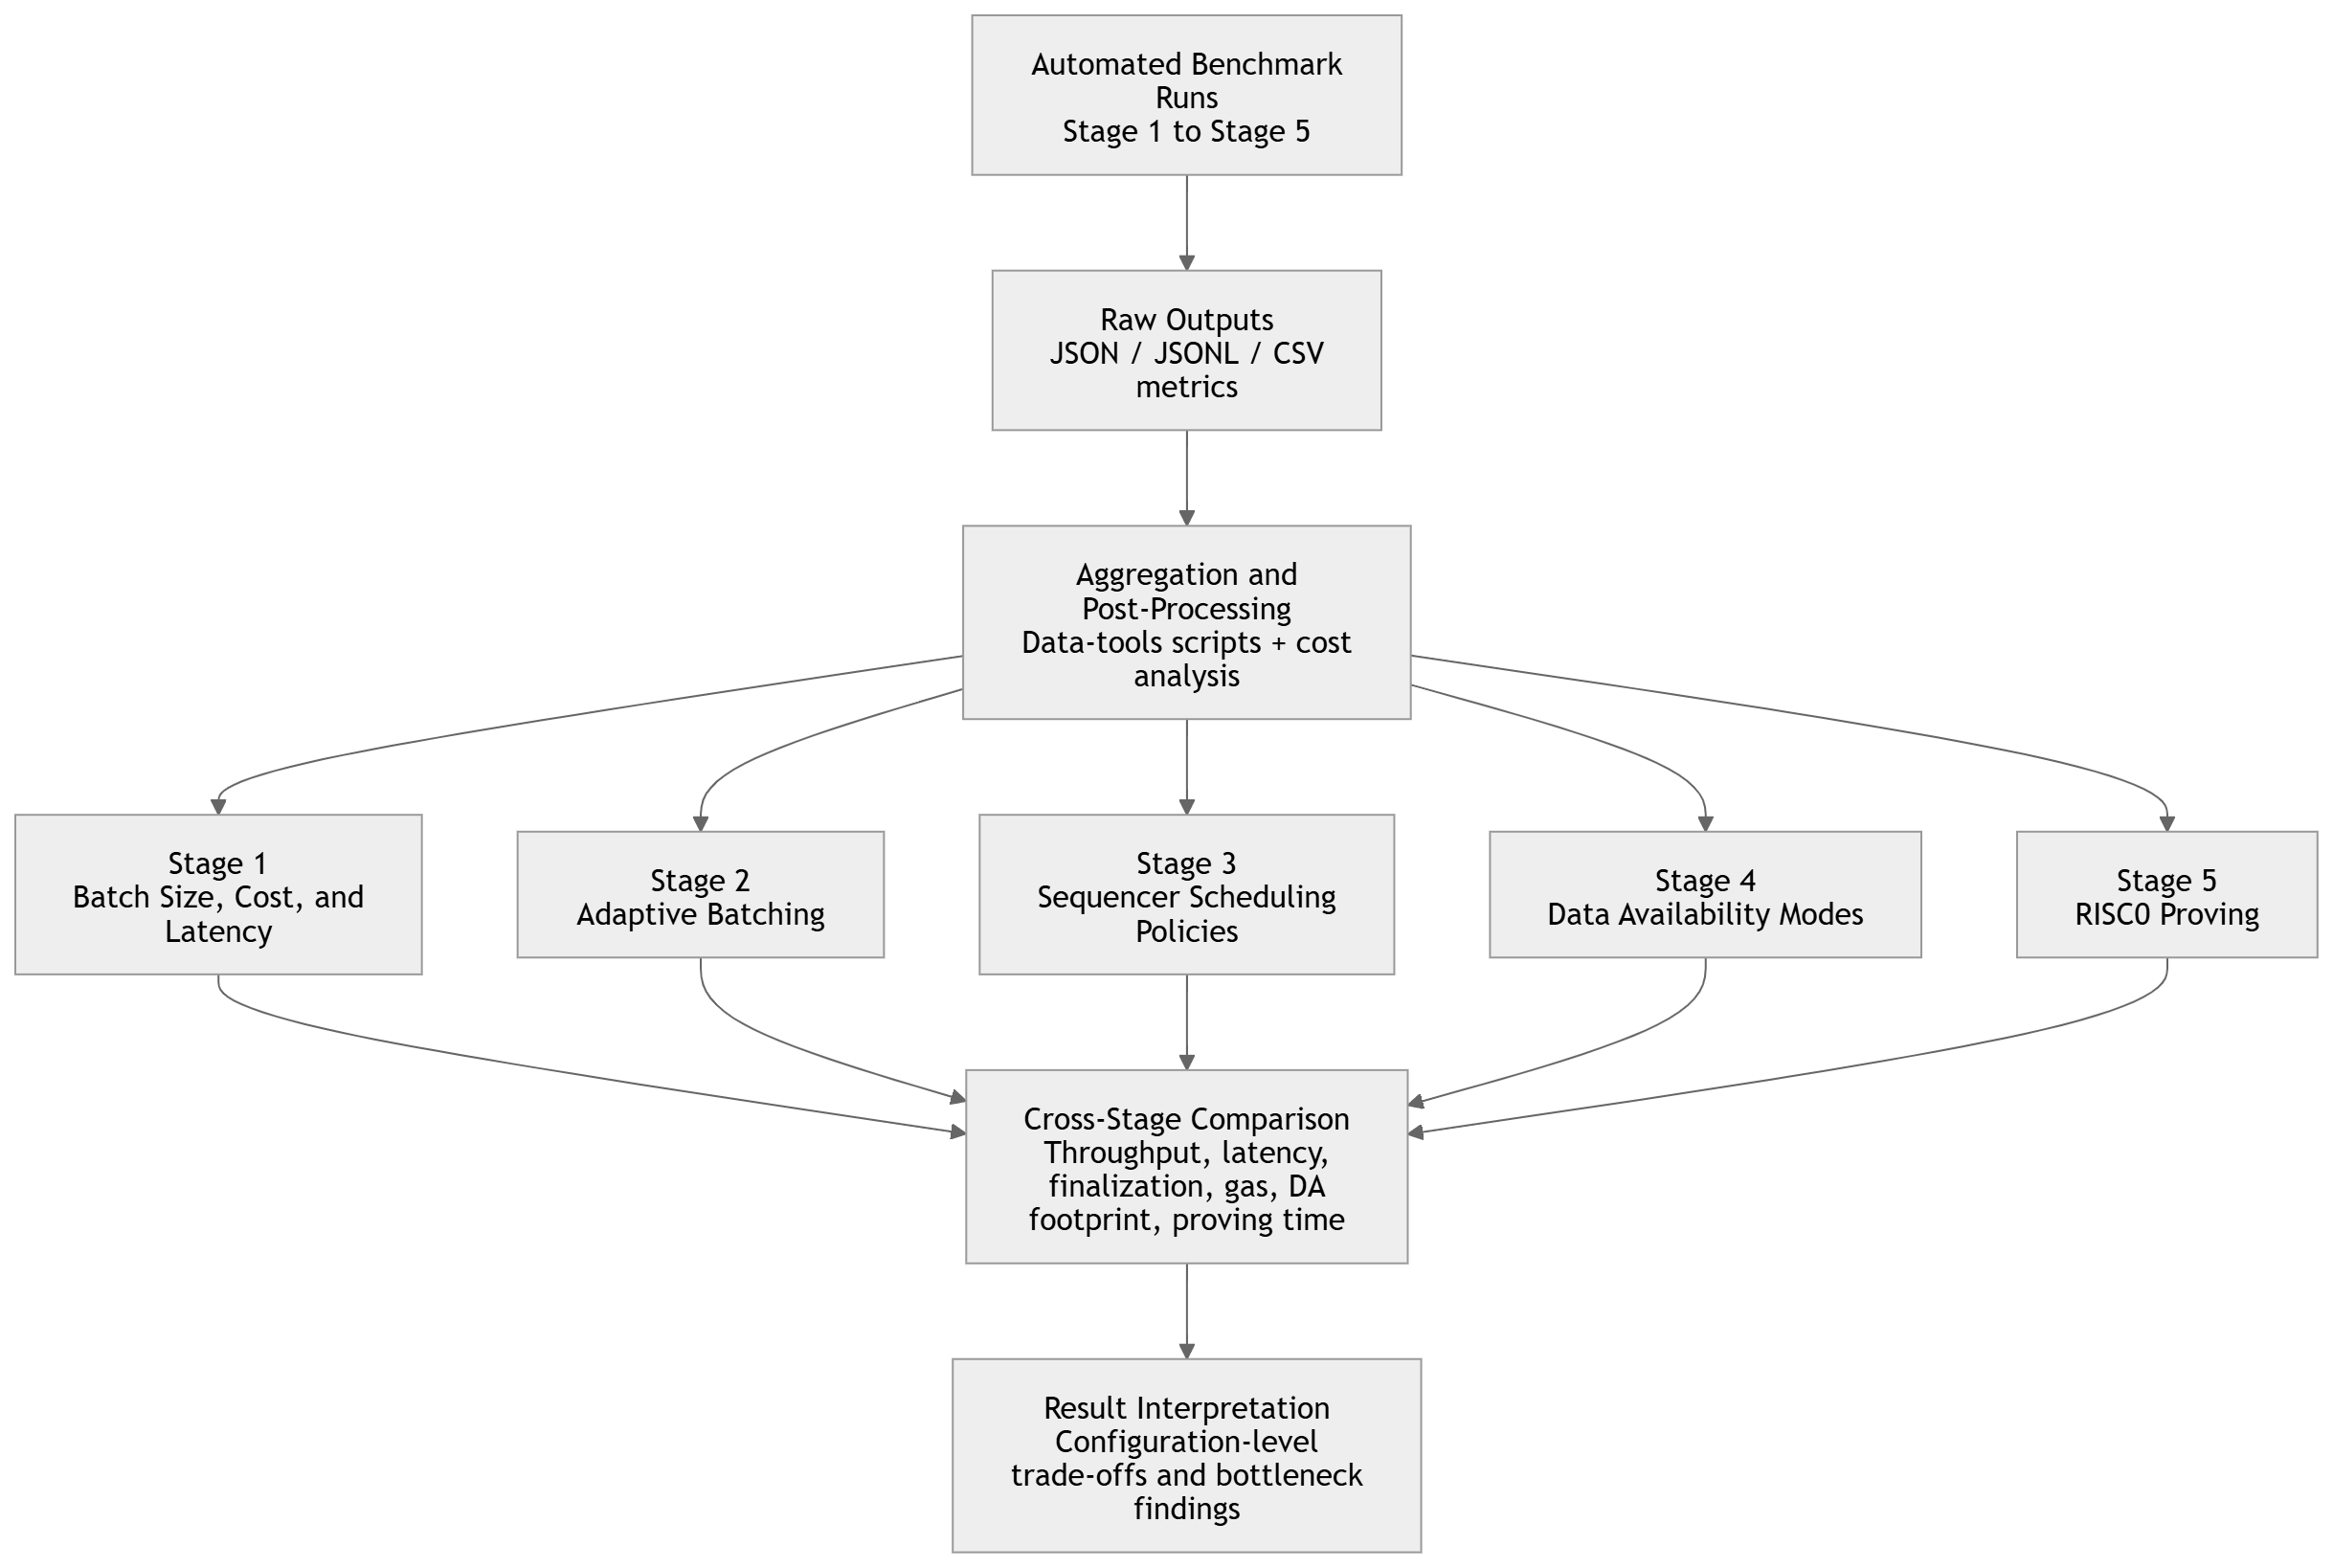
\includegraphics[
        width=0.82\textwidth,
        keepaspectratio
    ]{figures/chapter5/result_analysis_pipeline.png}
    \caption{Result-analysis pipeline used to organize and interpret the automated benchmark outputs.}
    \label{fig:result_analysis_pipeline}
\end{figure}

\subsection{Overview of Evaluation Stages}

As shown in Figure~\ref{fig:result_analysis_pipeline}, the empirical evaluation is structured into five stages, each focusing on a different aspect of the RollupX design space:

\begin{itemize}
    \item \textbf{Stage 1: Batch Size, Cost, and Latency.} This stage evaluates the fundamental trade-off between latency and cost using fixed batch sizes and timeout settings.

    \item \textbf{Stage 2: Adaptive Batching.} This stage evaluates dynamic batch scaling based on mempool load and threshold settings, with particular focus on whether adaptive batching can reduce queueing latency under varying traffic levels.

    \item \textbf{Stage 3: Sequencer Scheduling Policies.} This stage compares transaction ordering policies, such as FCFS, FairBFT, FeePriority, and TimeBoost, to study their effect on fairness, latency, and throughput under a nonce-aware scheduler design.

    \item \textbf{Stage 4: Data Availability (DA) Modes.} This stage analyzes the Layer-1 cost and payload implications of Calldata, Blob (EIP-4844-style), and Off-chain DA modes.

    \item \textbf{Stage 5: RISC0 Proving.} This stage profiles the computational overhead of real proof generation, including fixed setup overheads, segment boundaries, and cycle-dependent proving delay.
\end{itemize}

Together, these five stages provide a structured view of the major trade-offs in the prototype. The complete dataset representing the experimental configurations evaluated across these stages is summarized in Table~\ref{tab:results}.


\begin{table*}[htbp]
	\centering
	\caption{Comparative Performance Metrics Across Experimental Configurations}
	\label{tab:results}
	
oindent\resizebox{\textwidth}{!}{%
		\begin{tabular}{lllcrrrrrr}
			\toprule
			\textbf{Experimental Group} & \textbf{Configuration} & \textbf{Policy} & \textbf{DA Mode} & \textbf{Avg. Batch Size ($N$)} & \textbf{Throughput (TPS)} & \textbf{Wait Time (ms)} & \textbf{L1 Gas/Tx} & \textbf{Prove Time (s)} & \textbf{Cost/Tx (USD)} \\
			\midrule
			\multicolumn{10}{l}{\textit{Data Availability Mode Sweep (TPS-Adjusted Benchmark)}} \\
			DA Sweep: Calldata & Calldata ($N=22$) & FCFS & Calldata & 22.20 & 2.08 & 615 & 20,956 & 0.0 & \$0.6287 \\
			& Calldata ($N=45$) & FCFS & Calldata & 44.78 & 4.17 & 404 & 20,128 & 0.0 & \$0.6038 \\
			& Calldata ($N=72$) & FCFS & Calldata & 72.00 & 8.33 & 627 & 19,830 & 0.0 & \$0.5949 \\
			& Calldata ($N=132$) & FCFS & Calldata & 131.50 & 16.67 & 647 & 19,620 & 0.0 & \$0.5886 \\
			& Calldata ($N=290$) & FCFS & Calldata & 289.90 & 41.67 & 694 & 19,502 & 0.0 & \$0.5851 \\
			\midrule
			DA Sweep: Blob & Blob ($N=22$) & FCFS & Blob & 22.40 & 2.08 & 459 & 5,349 & 0.0 & \$0.1780 \\
			& Blob ($N=45$) & FCFS & Blob & 44.67 & 4.17 & 431 & 2,687 & 0.0 & \$0.0894 \\
			& Blob ($N=72$) & FCFS & Blob & 71.50 & 8.33 & 637 & 1,676 & 0.0 & \$0.0558 \\
			& Blob ($N=130$) & FCFS & Blob & 130.00 & 16.67 & 653 & 922 & 0.0 & \$0.0307 \\
			& Blob ($N=264$) & FCFS & Blob & 263.55 & 41.67 & 635 & 454 & 0.0 & \$0.0151 \\
			\midrule
			DA Sweep: Off-chain & Off-chain ($N=22$) & FCFS & Off-chain & 22.30 & 2.08 & 425 & 5,258 & 0.0 & \$0.1578 \\
			& Off-chain ($N=45$) & FCFS & Off-chain & 44.56 & 4.17 & 434 & 2,636 & 0.0 & \$0.0791 \\
			& Off-chain ($N=72$) & FCFS & Off-chain & 72.20 & 8.33 & 636 & 1,624 & 0.0 & \$0.0487 \\
			& Off-chain ($N=130$) & FCFS & Off-chain & 130.10 & 16.67 & 637 & 901 & 0.0 & \$0.0270 \\
			& Off-chain ($N=289$) & FCFS & Off-chain & 289.40 & 41.67 & 699 & 405 & 0.0 & \$0.0122 \\
			\midrule
			\multicolumn{10}{l}{\textit{Batch Policy Comparison (Fixed vs. Adaptive under Varying Load)}} \\
			Batch Policy: Fixed & Low Load (5 TPS) & Fixed & Calldata & 8.64 & 4.27 & 990 & 23,764 & 0.0 & \$0.7129 \\
			& Medium Load (25 TPS) & Fixed & Calldata & 36.70 & 18.58 & 994 & 20,200 & 0.0 & \$0.6060 \\
			& High Load (60 TPS) & Fixed & Calldata & 95.65 & 59.08 & 896 & 19,712 & 0.0 & \$0.5914 \\
			& Burst Load (8 TPS) & Fixed & Calldata & 52.11 & 25.98 & 976 & 20,005 & 0.0 & \$0.6002 \\
			\midrule
			Batch Policy: Adaptive & Low Load (5 TPS) & Adaptive & Calldata & 2.41 & 4.25 & 252 & 55,882 & 0.0 & \$1.6765 \\
			& Medium Load (25 TPS) & Adaptive & Calldata & 9.23 & 18.10 & 259 & 22,974 & 0.0 & \$0.6892 \\
			& High Load (60 TPS) & Adaptive & Calldata & 48.44 & 59.08 & 450 & 20,009 & 0.0 & \$0.6003 \\
			& Burst Load (8 TPS) & Adaptive & Calldata & 16.34 & 25.98 & 293 & 22,832 & 0.0 & \$0.6850 \\
			\midrule
			\multicolumn{10}{l}{\textit{Sequencer Scheduling Ordering Comparison (Normal Load)}} \\
			Sequencer Order & FCFS & FCFS & Calldata & 36.84 & 19.85 & 1,004 & 20,200 & 0.0 & \$0.6060 \\
			& FairBFT & FairBFT & Calldata & 36.98 & 19.93 & 1,012 & 20,190 & 0.0 & \$0.6057 \\
			& FeePriority & FeePriority & Calldata & 35.97 & 6.59 & 1,020 & 20,261 & 0.0 & \$0.6078 \\
			& TimeBoost & TimeBoost & Calldata & 35.76 & 6.56 & 1,028 & 20,239 & 0.0 & \$0.6072 \\
			\midrule
			\multicolumn{10}{l}{\textit{zkVM Proof Generation Constraints}} \\
			zkVM Proving & zkVM ($N=50$) & FCFS & Calldata & 42.17 & 1.41 & 7,333 & 20,385 & 317.8 & \$0.6115 \\
			& zkVM ($N=100$) & FCFS & Calldata & 83.00 & 1.38 & 37,660 & 19,755 & 540.8 & \$0.5926 \\
			& zkVM ($N=200$) & FCFS & Calldata & 126.00 & 1.40 & 47,779 & 19,615 & 782.4 & \$0.5884 \\
			& zkVM ($N=500$) & FCFS & Calldata & 246.00 & 1.37 & 119,204 & 19,503 & 1,487.3 & \$0.5851 \\
			\bottomrule
		\end{tabular}%
	}
\end{table*}
\subsection{Validation of Scheduling and Batching Designs}
The empirical results successfully validated the key components of the modular ZK-Rollup prototype:
\begin{itemize}
    \item \textbf{Nonce-Aware Scheduler Validation:} Under the benchmark runs, the priority scheduling policies (\texttt{FeePriority} and \texttt{TimeBoost})—which group transactions by account and sort them strictly by nonce—executed all transactions successfully with 100\% transaction execution success (0 empty batches), yielding FCFS-equivalent regular gas costs (~20.2k gas/tx). Furthermore, under burst workloads, TimeBoost achieved a Jain's Fairness Index of \textbf{0.77}, outperforming standard FeePriority and FCFS policies by confining fee-based prioritization to discrete 5-second windows.
    \item \textbf{Adaptive Batching Performance:} Under low offered load (5 TPS), the adaptive batching policy successfully reduced mempool queue latency to 252 ms, although with a corresponding increase in gas cost per transaction as expected by the cost model.
    \item \textbf{Production zkVM Prover Profiling:} Real RISC0 prover sweeps validated the computational proving bottlenecks, demonstrating linear cycle scaling with segment-based step-function proving delays and a constant 256-byte proof footprint.
\end{itemize}
